\chapter{Video Input}

\section{Beeldformaat}
	\subsection{Video frame}
		\par De video input is een stream van frames die elk een beeld voorstellen. De NTSC standaard, gedefinieerd volgens ITU-R BT656~\cite{bib_3}~\cite{bib_4}, legt een framerate van 60Hz op, dus 60 frames per seconde. Elk frame bestaat uit verschillende lijnen data, zichtbare en onzichtbare. De zichtbare lijnen zijn gegroepeerd per even en oneven regels, en zijn dus in twee velden, Active Video Fields (AVF), terug te vinden in het binnekomende frame. De overige, en dus onzichtbare lijnen, zorgen voor synchronisatie tussen de bron en de weergever. Deze regels worden ook blanking lines genoemd. Hoe de lijnen precies voorkomen in een frame is te vinden in figuur~\ref{fig:OpbouwFrameImage}.
		
		\begin{figure}[H]
			\centering
			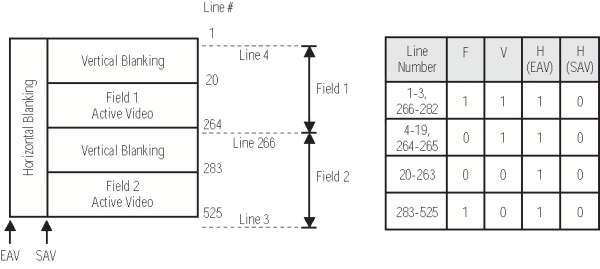
\includegraphics[width=0.95\textwidth]{Chapters/Chapter1/Images/Frame.png}
			\caption{Opbouw ITU-R BT656 frame~\cite{bib_15}}
			\label{fig:OpbouwFrameImage}
		\end{figure}

		\par Er is duidelijk te zien dat er eerst een groep lijnen komt die de vertical blanking lijnen voorstellen. Deze regels gaven de vroegere CRT televisietoestellen de tijd om hun beam van beneden tot weer volledig boven te bewegen. Aangezien de nieuwere toestellen niet meer met een kathodestraalbuis werken, maar over een volledig digitaal verwerkingssysteem beschikken, kan deze data overschreven worden met timingintervallen of andere metadata. Er kan dus data meegestuurd worden binnenin de blanking intervallen, maar deze wordt door vele toestellen uitgefilterd om interferentie van beeldlijnen te voorkomen.

		\par De vertical blanking is opgevolgd door het eerste AVF. Deze eerste groep bevat de oneven lijnen van het zichtbare beeld.
		Hoe een lijn precies in elkaar zit wordt in het volgende onderdeel verder beschreven, hier beperken we ons tot de adressering van de lijnen binnen het frame. Dit eerste AVF is gevolgd door opnieuw een vertical blanking en een AVF. Een ITU-R BT656 frame bestaat uit 525 opeenvolgende lijnen. Aangezien het zictbare beeld 480 lijnen telt, blijven er 48 lijnen over die kunnen dienen voor vertical blanking, wat duidelijk overeenkomt met figuur~\ref{fig:OpbouwFrameImage} op pagina ~\pageref{fig:OpbouwFrameImage}.

	\subsection{Structuur van een beeldlijn}
	\label{subsec:LijnSubSec}
		\par Er zijn twee soorten lijnen, de zichtbare en de onzichtbare. Ze delen eenzelfde opbouw, maar hebben een groot verschil, namelijk dat de zichbare lijnen een AVF bevatten waar de onzichtbare lijnen een vertical blanking field bevatten. Zowel de headers als de lijnlengte zijn exact gelijk en kunnen dus beschouwd worden als eenzelfde opeenvolging van data. Men moet er bij het verwerken wel voor zorgen dat er niet over de vertical blanking geschreven wordt op willekeurige plaatsen, omdat dit ongewenste effecten kan hebben, afhankelijk van het type toestel waarop het beeld weergegeven wordt.

		\begin{figure}[H]
			\centering
			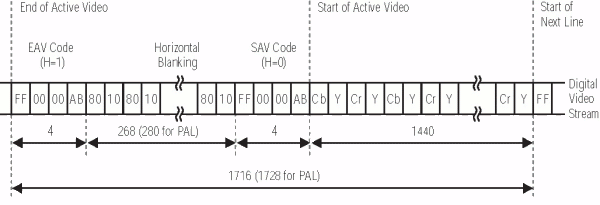
\includegraphics[width=0.95\textwidth]{Chapters/Chapter1/Images/Line.png}
			\caption{Opbouw ITU-R BT656 lijn ~\cite{bib_16}}
			\label{fig:OpbouwLijnImage}
		\end{figure}

		\par Een lijn bestaat uit verscheidene elementen: EAV code, horizontal blanking, SAV code en data. De EAV code heeft een lengte van 4 bytes en bestaat uit drie bytes met een vaste waarde (0xFF 0x00 0x00), gevolgd door een vierde byte die aanduidt of de data die volgt bestaat uit de even of oneven lijnen, alsook de status van de blanking. Op deze manier weet het toestel of de lijn een blanking, al dan niet een beeldlijn voorstelt. De blanking die erop volgt is opgebouwd uit een continue opvolging van 0x80 0x10, en dit voor een lengte van 268 bytes. Deze data zorgt voor de horizontale uitlijning van het beeld. De SAV code staat voor Start of Active Video en dient dus om aan te tonen dat de een AVF zal starten zodra de SAV code voorbij is. Deze heeft opnieuw een lengte van 4 bytes, bestaande uit drie vaste bytes (0xFF 0x00 0x00) gevolgd door een code die aanduidt welke data er zal volgen, zijnde welk field (even of oneven) en de blanking status.
		Als laatste is er dus de effectieve lijndata, met een lengte van 1440 bytes. Deze 1440 bytes stellen een volledige lijn voor, zij het even of oneven, en tellen dus 720 pixels, wat neerkomt op 2 bytes per pixel. Er is een opvolging van Cb Y Cr Y over de volledige lengte, hoe dit formaat precies gestructureerd is wordt in het volgende hoofdstuk besproken.

\section{Kleurenruimte}
	\subsection{RGB}
		\par RGB is de meest gekende en voor de hand liggende kleurenruimte, ze bestaat uit een combinatie van de 3 kleuren Rood, Groen en Blauw en is voor de gebruiker ook de meest eenvoudige manier om een kleur te omschrijven. Er bestaan echter verschillende formaten van deze RGB standaard, vaak gekozen om datacompressie toe te passen waar mogelijk. Als we RGB als een 24 bits getal zien van telkens 8 bits per kleurwaarde, kunnen we heel eenvoudig een kleur detecteren en deze aanpassen. Cfr.~\ref{subsec:KleurConversieSubSec} voor de omzetting van RGB naar YCbCr en omgekeerd. Op figuur~\ref{fig:RGBColorSpaceImage} is te zien hoe deze kleurruimte kan worden voorgesteld.

		\par Een kleur aanpassen in deze ruimte is vrij voor de hand liggend, aangezien het een voorstelling is die we gewoon zijn. We kunnen de componenten namelijk perfect apart waarnemen en ons voorstellen. Op die manier kunnen we dan ook meteen voor ons zien wat er zal gebeuren als een aanpassing zouden doen aan \'e\'en van de componenten.

		\begin{figure}[H]
			\centering
			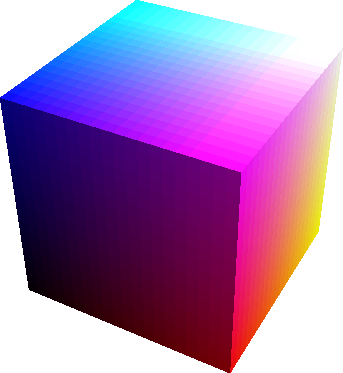
\includegraphics[width=0.35\textwidth]{Chapters/Chapter1/Images/RGBspace.png}
			\caption{RGB kleurenruimte~\cite{bib_17}}
			\label{fig:RGBColorSpaceImage}
		\end{figure}
		
		\par Stel dat we een RGB kleur (97,179,254) hebben, en we willen hierop een transformatie uitvoeren dan hebben we reeds alle kleuren ter beschikking. Indien we de helderheid willen opdrijven moeten we alle drie de waarden aanpassen, namelijk verhogen met eenzelfde factor. Het tegenovergestelde geldt voor het verdonkeren van de kleur.
		\par Willen we een kleurverandering doorvoeren, zoals dit met deze opdracht het geval is met blauw en geel, blijft dit toch nog een vrij complexe operatie. In het geval we blauw willen converteren naar geel moeten we de rode en de groene component vergroten terwijl we de blauwe component drastisch laten inkrimpen. In pseudocode kan dit verwezenlijkt worden op de volgende manier:
		\bigskip
   		\begin{lstlisting}[language=VBScript, caption=Pseudocode voor het vervangen van blauw met geel]
if 0>R>115 and 100>G>200 and 0>B>255
   	R = 255
   	G = 255
   	B = 0
end		\end{lstlisting}

		Dit levert echter een monotoon geel op, wat voor de ogen niet zo aangenaam is om naar te kijken. Daarom kiezen we om de (R,G,B) componenten geen exacte nieuwe waarde te geven, maar \'e\'en die afhankelijk is van hun oorspronkelijke waarde. Dit kunnen we doen door de waarden met een vaste maat te vergroten of verkleinen, vertrekken van de waarde die de pixel reeds heeft.
		\bigskip
		\begin{lstlisting}[language=VBScript, caption=Pseudocode voor het vervangen van blauw met geel met behoud van tinten]
if 0>R>115 and 100>G>200 and 0>B>255
	R = 255
	G = min(G+54, 255)
	B = max(B-215,0)
end		\end{lstlisting}

	\newpage
	\subsection{YCbCr}
	\label{subsec:YCbCrSubSec}
		\par YCbCr is geen echte kleurenruimte, maar een formaat om een kleurenruimte te transporteren van een bron naar een scherm, het is gebruikt in het ITU-R BT656 formaat en is ontworpen om een zelfde kleurervaring te leveren in slechts 16 bits per pixel in plaats van 24 bij standaard RGB. Eigenlijk is het niet volledig correct om van 16 bits per pixel te spreken, aangezien we eigenlijk 32 bits per 2 pixels gebruiken~\cite{bib_2}. Twee naast elkaar liggende pixels delen eenzelfde Cb en Cr waarde, terwijl ze elk een eigen Y-waarde bevatten. Het menselijk oog is namelijk veel gevoeliger voor veranderingen in helderheid dan voor veranderingen in kleur. Op figuur~\ref{fig:YCbCrColorSpaceImage} is te zien hoe deze kleurruimte kan worden voorgesteld.

		\begin{figure}[H]
			\centering
			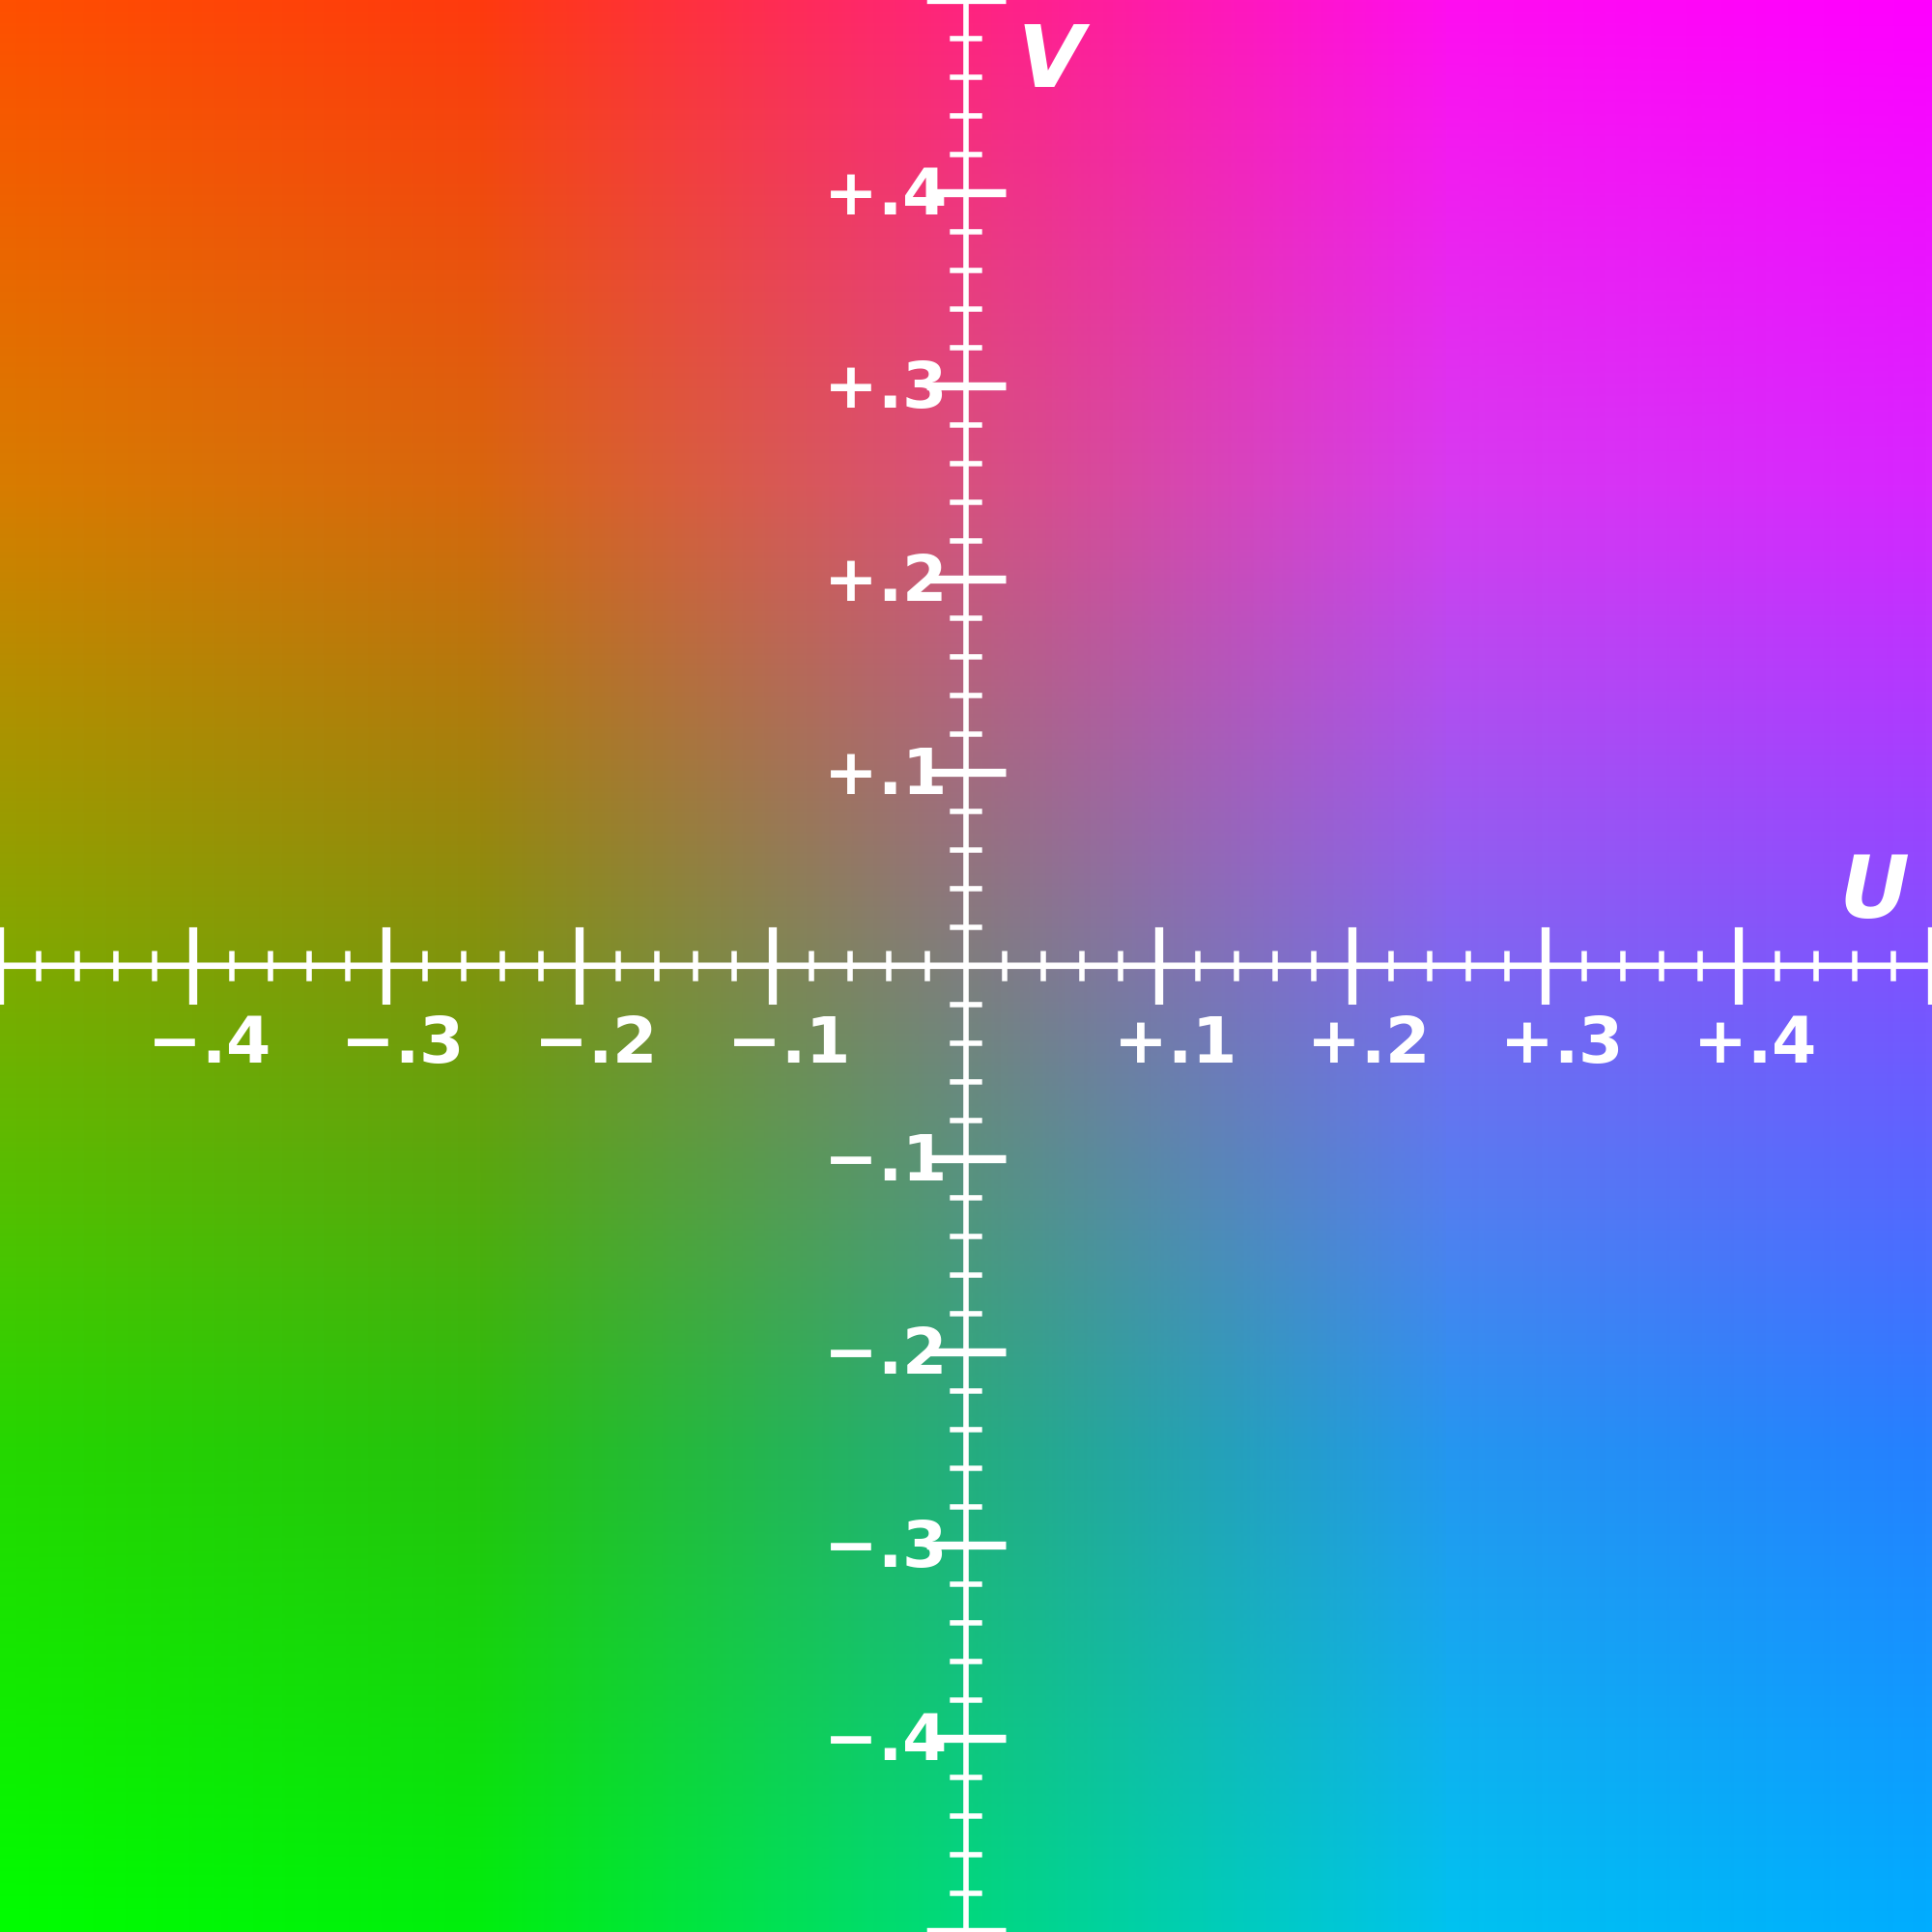
\includegraphics[width=0.4\textwidth]{Chapters/Chapter1/Images/YUVspace.png}
			\caption{YCbCr Kleurenruimte~\cite{bib_18}}
			\label{fig:YCbCrColorSpaceImage}
		\end{figure}

		\par Het vervangen van een kleur in het YCbCr formaat is heel wat complexer omdat het kleurenbereik dat we nodig hebben om een Smurf volledig naar geel te wijzigen, zo groot is dat we andere kleuren ook mee converteren. Grijstinten zijn een voorbeeld van deze bijkomende kleuren. Het afstellen van het bereik is dus veel preciezer, maar door te precies te werk te gaan verliezen we een deel van het blauwe spectrum waardoor de kans bestaat dat niet alle blauw gezien wordt als binnen de grenzen liggend. Het algoritme ziet er in pseudocode als volgt uit:
		\bigskip
		\begin{lstlisting}[language=VBScript, caption=Pseudocode voor het vervangen van blauw door geel]
if Y >= 130 and Y <= 180 and Cb > 150 and Cr > 50 and Cr < 100)
	Y = 0xEB
	Cb = 0x28
	Cr = 0x98
end		\end{lstlisting}

	\subsection{Conversie}
	\label{subsec:KleurConversieSubSec}
		\par Voor de conversie van RGB naar YCbCr en omgekeerd zijn er enkele vaste formules die gehanteerd kunnen worden. Aan de hand van de samenstelling van een lijn kunnen we dus uit 4 bytes data van het Active Video Frame 2 pixels halen. Deze waarden kunnen dan via de volgende formules~\cite{bib_1} geconverteerd worden tussen beide formaten:
   		
   		\begin{table}[H]
			\centering
				\begin{tabular}{@{}l|l@{}}
					\toprule
					RGB to YCbCr&YCbCr to RGB  \\ \midrule
					$R = Y + 1.140V$&$Y =  0.299R + 0.587G + 0.114B$ \\
					$G = Y - 0.395U - 0.581V$&$U = -0.147R - 0.289G + 0.436B$  \\
					$B = Y + 2.032U$&$V =  0.615R - 0.515G - 0.100B$ \\ \bottomrule
				\end{tabular}
			\caption{Formules RGB en YCbCr conversie ~\cite{bib_1}}
			\label{tab:RGBYCbCrFormulesTable}
		\end{table}

		\par Kleurenconversie tussen deze twee ruimtes is dus prefect mogelijk in beide richtingen. In ideale omstandigheden kunnen we dus voor deze opdracht de YCbCr waardes binnenlezen voor twee naast elkaar liggende pixels, en deze converteren naar twee RGB pixels. We laten het algoritme om de blauwe kleur te veranderen in geel inwerken op beide van deze pixels, en converteren deze opnieuw naar de YCbCr ruimte om ze dan terug in het frame te plaatsen en weer uit te sturen.
		\bigskip
		\begin{lstlisting}[language=VBScript,caption=Pseudocode voor een kleurconversie en -vervanging van blauw naar geel]
R = Y + 1.140V
G = Y - 0.395U - 0.581V
B = Y + 2.032U

if 0>R>115 and 100>G>200 and 0>B>255
	R = 255
	G = min(G+54, 255)
	B = max(B-215,0)
end

Y =  0.299R + 0.587G + 0.114B
U = -0.147R - 0.289G + 0.436B
V =  0.615R - 0.515G - 0.100B		\end{lstlisting}

		\par Na wat experimenteren zijn we echter tot de conclusie gekoment dat deze ideale omstandigheden niet bestaan, of toch niet in deze situatie. De processor is namelijk niet in staat om binnen de tijd van \'e\'en enkel frame over alle pixels te itereren en deze conversie uit te voeren. Aangezien het omzetten gebruikt maakt van floating point operaties neemt dit te veel tijd in beslag om op tijd klaar te zijn. Het zal dus noodzakelijk zijn om de kleurwijziging uit te voeren binnen de YCbCr kleurenruimte. Dit brengt echter heel wat nadelen met zich mee, cfr.~\ref{subsec:YCbCrSubSec} op pagina~\pageref{subsec:YCbCrSubSec}.

\section{Kleurbepaling van een Smurf}

	\par De kleur van een Smurf werd aan de hand van het programma Photoshop bepaald in de RGB kleurenruimte. Een Smurf heeft geen solide kleur dus werd er een bereik bepaald waarbinnen een kleur moet vallen om als Smurfenblauw gedetecteerd te worden. Deze RGB kleurwaarden werden door middel van het programma Matlab geconverteerd naar de YCbCr kleurenruimte volgens de formules die eerder in dit hoofdstuk besproken werden. De grenzen worden weergegeven in tabel~\ref{tbl:huidskleurwaarden}.

		\begin{table}[h]
			\centering
			\begin{tabular}{l|cc}
			\multicolumn{1}{c}{} & Minimum waarde & Maximum waarde \\
			\hline
			Y                    & 130            & 180            \\
			Cb                   & 150            & 240            \\
			Cr                   & 50             & 100            \\
			\hline
			\hline
			R                    & 8              & 146            \\
			G                    & 187            & 170            \\
			B                    & 177            & 255        	   \\
			\hline   
			\end{tabular}
		\caption{Bereik van de huidskleurwaarden van een Smurf}
		\label{tbl:huidskleurwaarden}
		\end{table}

